
%(BEGIN_QUESTION)
% Copyright 2007, Tony R. Kuphaldt, released under the Creative Commons Attribution License (v 1.0)
% This means you may do almost anything with this work of mine, so long as you give me proper credit

%This control strategy for liquid level control is called {\it feedforward with trim}, {\it feedforward-feedback} control, or {\it three-element} control:
Denne reguleringsmetoden for niv{\aa}kontroll blir kalt treelements regulering. 

$$\includegraphics[width=15.5cm]{i01750x01.eps}$$
%What will this system do to maintain a constant level in the vessel if the ``wild'' flow input to the vessel suddenly increases?
Hva vil dette systemet gj{\o}re for {\aa} holde konstant niv{\aa} hvis det er store variasjoner str{\o}mning inn i tanken. 
\vskip 10pt

%Also, what will this system do to maintain a constant liquid level if a leak suddenly develops in the vessel?
Og hva vil systemer gj{\o}re for {\aa} holde konstant niv{\aa}, om det oppst{\aa}r en lekkasje i tanken?
\vskip 20pt \vbox{\hrule \hbox{\strut \vrule{} {\bf Suggestions for Socratic discussion} \vrule} \hrule}

\medskip
\item{$\bullet$} Explain why pure feedforward control is almost never used in industry.  Instead, we almost always see feedforward used as part of a larger feedback control strategy.
\item{$\bullet$} A problem-solving technique useful for analyzing control systems is to mark the PV and SP inputs of all controllers with ``+'' and ``$-$'' symbols, rather than merely label each controller as ``direct'' or ``reverse'' action.  Apply this technique to the control strategy shown here, identifying which controller input(s) should be labeled ``+'' and which controller input(s) should be labeled ``$-$''.
\item{$\bullet$} Explain what will happen if the level transmitter fails with a low signal.
\item{$\bullet$} Explain what will happen if the level transmitter fails with a high signal.
\item{$\bullet$} Explain what will happen if the summing relay fails with a low signal.
\item{$\bullet$} Explain what will happen if the summing relay fails with a high signal.
\item{$\bullet$} Explain what will happen if the flow controller is left in manual mode.
\item{$\bullet$} Explain what will happen if the level controller is left in manual mode.
\item{$\bullet$} Explain what will happen if the wild flow transmitter fails with a low signal.
\item{$\bullet$} Explain what will happen if the wild flow transmitter fails with a high signal.
\item{$\bullet$} Explain what will happen if the captive flow transmitter fails with a low signal.
\item{$\bullet$} Explain what will happen if the captive flow transmitter fails with a high signal.
\medskip

\underbar{file i01750}
%(END_QUESTION)





%(BEGIN_ANSWER)

If the wild flow increases, the flow transmitter on that line will send an increased signal to the summer (FY), which will increase the setpoint to the outlet flow controller (FC), which will open the flow valve appropriately to handle the extra incoming flow, with no ``bump'' to the liquid level.

\vskip 10pt

If the vessel springs a leak, the level transmitter will register a decrease in liquid level, the level indicating controller (LIC) will output a lesser signal to the summer (FY), decreasing the setpoint sent to the flow controller (FC) and compensating for the extra load on the process.

%(END_ANSWER)





%(BEGIN_NOTES)

Ideally, the level controller will neither see any change in level, nor have to output a different signal to the summer.  The feedforward portion of this control system has compensated for the increase in ``wild'' flow.

\vskip 10pt

In the leak scenario, the feedback portion of the control system does all the compensation.  The feedforward portion of the system ``knows'' nothing of the leak in the vessel, so it cannot take any corrective action of its own.  Because the response in this case is feedback and not feedforward, the process variable (vessel level) will be ``bumped'' by the sudden presence of a leak.

\vskip 20pt \vbox{\hrule \hbox{\strut \vrule{} {\bf Virtual Troubleshooting} \vrule} \hrule}

This question is a good candidate for a ``Virtual Troubleshooting'' exercise.  Presenting the diagram to students, you first imagine in your own mind a particular fault in the system.  Then, you present one or more symptoms of that fault (something noticeable by an operator or other user of the system).  Students then propose various diagnostic tests to perform on this system to identify the nature and location of the fault, as though they were technicians trying to troubleshoot the problem.  Your job is to tell them what the result(s) would be for each of the proposed diagnostic tests, documenting those results where all the students can see.

During and after the exercise, it is good to ask students follow-up questions such as:

\medskip
\item{$\bullet$} What does the result of the last diagnostic test tell you about the fault?
\item{$\bullet$} Suppose the results of the last diagnostic test were different.  What then would that result tell you about the fault?
\item{$\bullet$} Is the last diagnostic test the best one we could do?
\item{$\bullet$} What would be the ideal order of tests, to diagnose the problem in as few steps as possible?
\medskip

%INDEX% Control, strategies: feedforward

%(END_NOTES)


